\documentclass[aspectratio=169,11pt]{beamer}

\usetheme{Madrid}
\usecolortheme{seahorse}

\usepackage[utf8]{inputenc}
\usepackage[T1]{fontenc}
\usepackage[brazil]{babel}
\usepackage{amsmath,amsthm,amssymb}
\usepackage{graphicx}
\usepackage{tikz}
\usetikzlibrary{shapes,arrows,positioning}

\title{Modelagem Geométrica}
\subtitle{Representações Celulares Adaptativas e Esferas Geodésicas}
\author{Relatório de Implementação}
\date{2 de Fevereiro de 2026}

\begin{document}

\begin{frame}
    \titlepage
\end{frame}

%=============================================================================
% SLIDE 1: Representação Adaptativa (Quadtree)
%=============================================================================
\begin{frame}{Representação Celular Adaptativa (Quadtree)}

\begin{columns}[T]
\begin{column}{0.45\textwidth}

\textbf{Princípio:} Subdividir apenas células que intersectam a fronteira

\vspace{0.2cm}

\textbf{Classificação de Células:}
\begin{itemize}
    \item $\sigma = 0$: Exterior (branco)
    \item $\sigma = 1$: Interior (azul)
    \item $\sigma = 2$: Interseção $\rightarrow$ \textbf{subdivide}
\end{itemize}

\vspace{0.2cm}

\textbf{Complexidade:} $O(L \cdot 2^d)$ células na fronteira

\end{column}

\begin{column}{0.52\textwidth}
\begin{center}
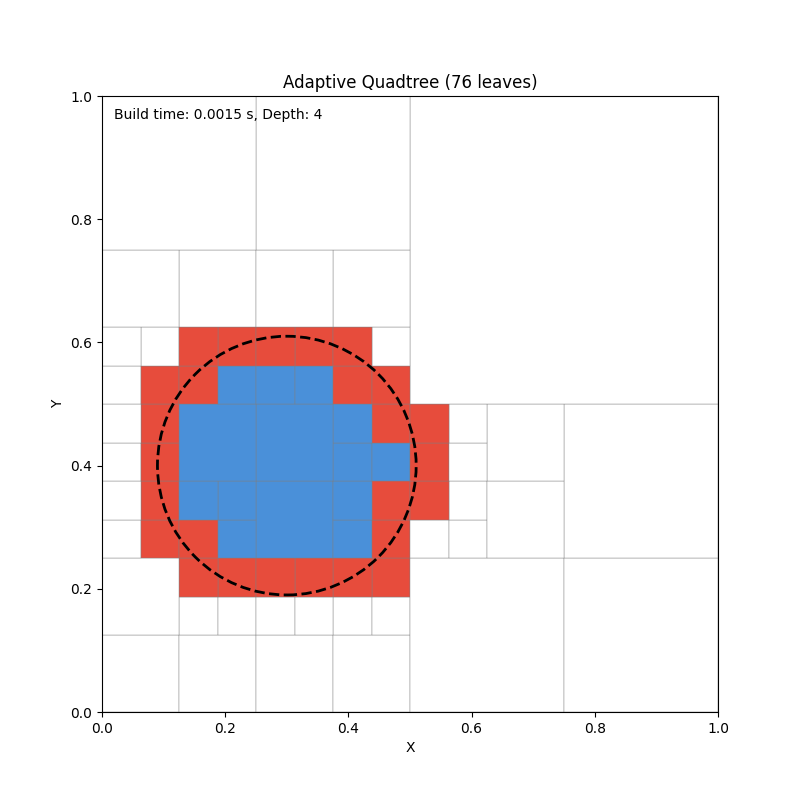
\includegraphics[width=0.48\textwidth]{../img/quadtree_circle_0_depth_4.png}
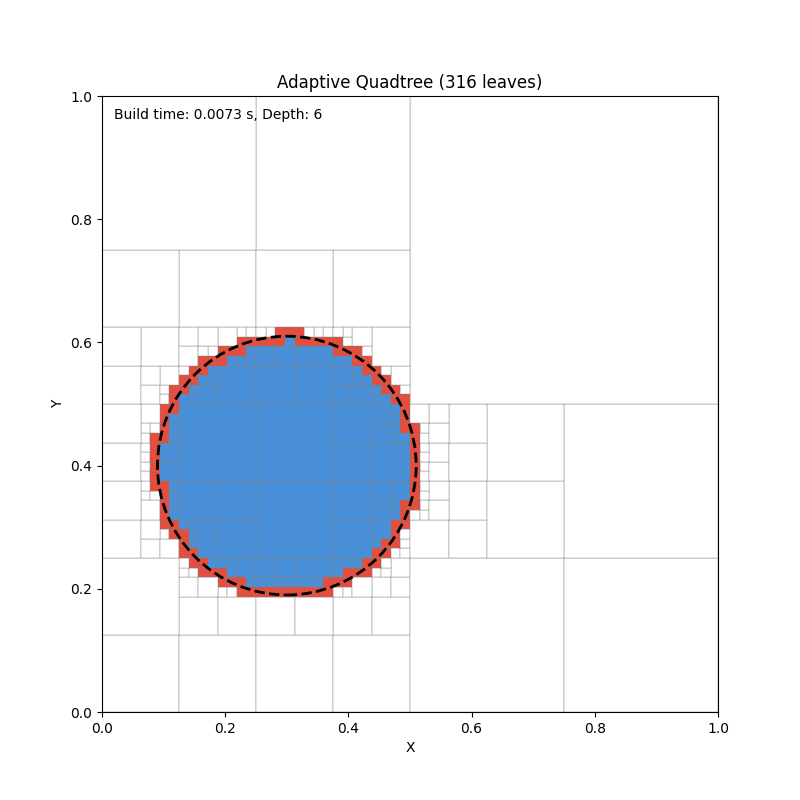
\includegraphics[width=0.48\textwidth]{../img/quadtree_circle_0_depth_6.png}

\vspace{0.1cm}
\footnotesize Disco: profundidade 4 (esq.) e 6 (dir.)
\end{center}
\end{column}
\end{columns}

\vspace{0.2cm}

\begin{block}{Algoritmo}
\texttt{if classify(cell) == INTERSECT and depth < max\_depth: subdivide(cell)}
\end{block}

\end{frame}

%=============================================================================
% SLIDE 2: Refinamento da Esfera Geodésica
%=============================================================================
\begin{frame}{Esfera Geodésica por Refinamento}

\begin{columns}[T]
\begin{column}{0.42\textwidth}

\textbf{Entrada:} Icosaedro (12 vértices, 20 faces)

\vspace{0.2cm}

\textbf{Algoritmo:}
\begin{enumerate}
    \item Calcular pontos médios: $m_{ij} = \frac{v_i + v_j}{2}$
    \item Projetar na esfera: $m'_{ij} = \frac{m_{ij}}{\|m_{ij}\|}$
    \item Criar 4 novos triângulos
\end{enumerate}

\vspace{0.2cm}

\textbf{Crescimento:} $F_k = 4^k \cdot F_0$

\end{column}

\begin{column}{0.55\textwidth}
\begin{center}
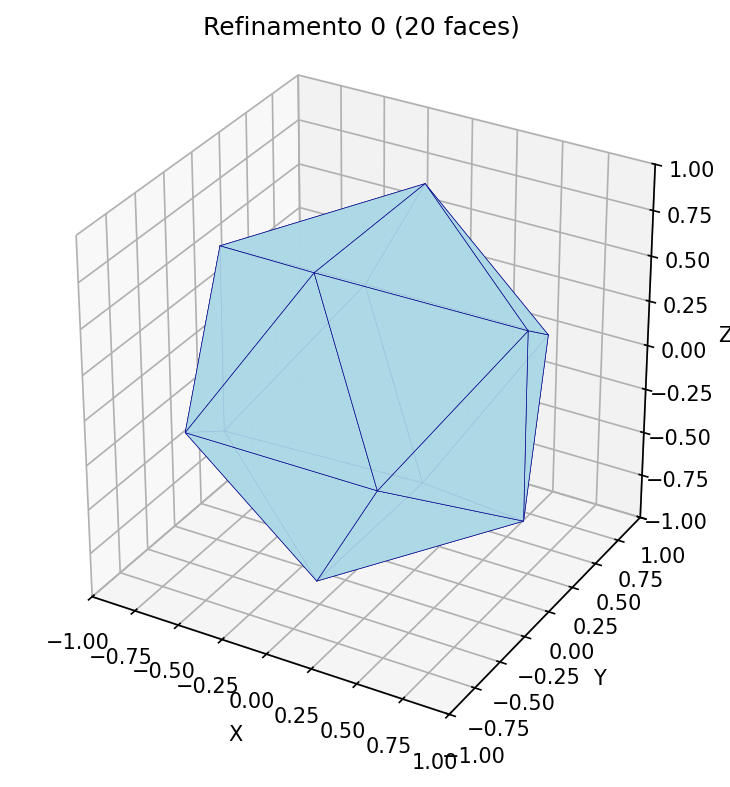
\includegraphics[width=0.48\textwidth]{../img/sphere_refine_0.png}
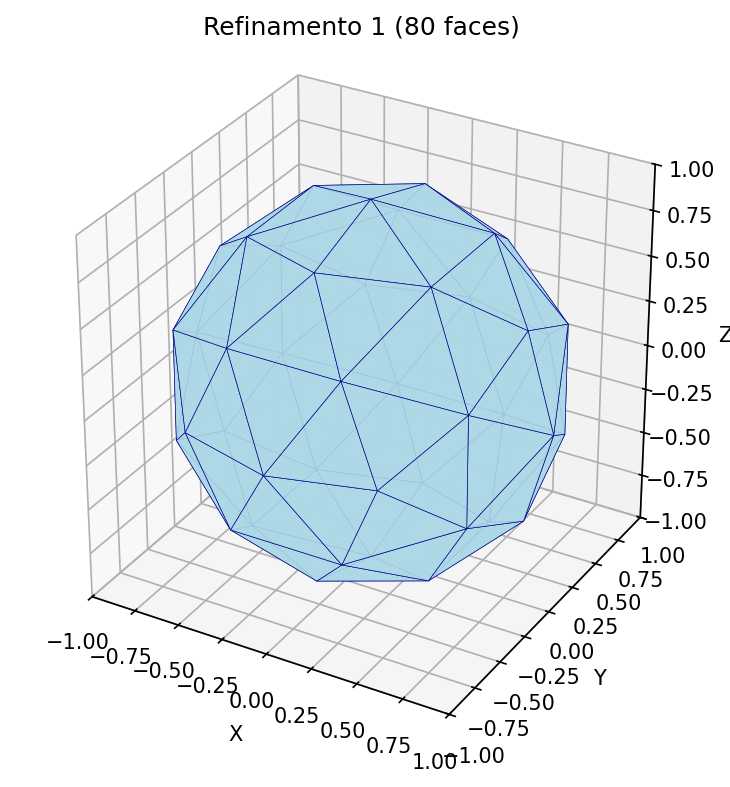
\includegraphics[width=0.48\textwidth]{../img/sphere_refine_1.png}

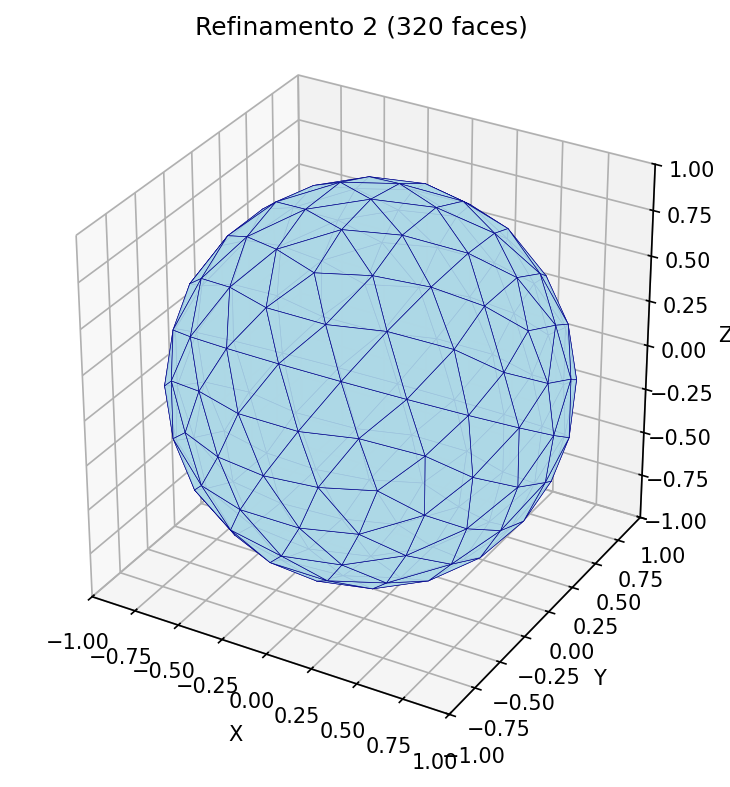
\includegraphics[width=0.48\textwidth]{../img/sphere_refine_2.png}
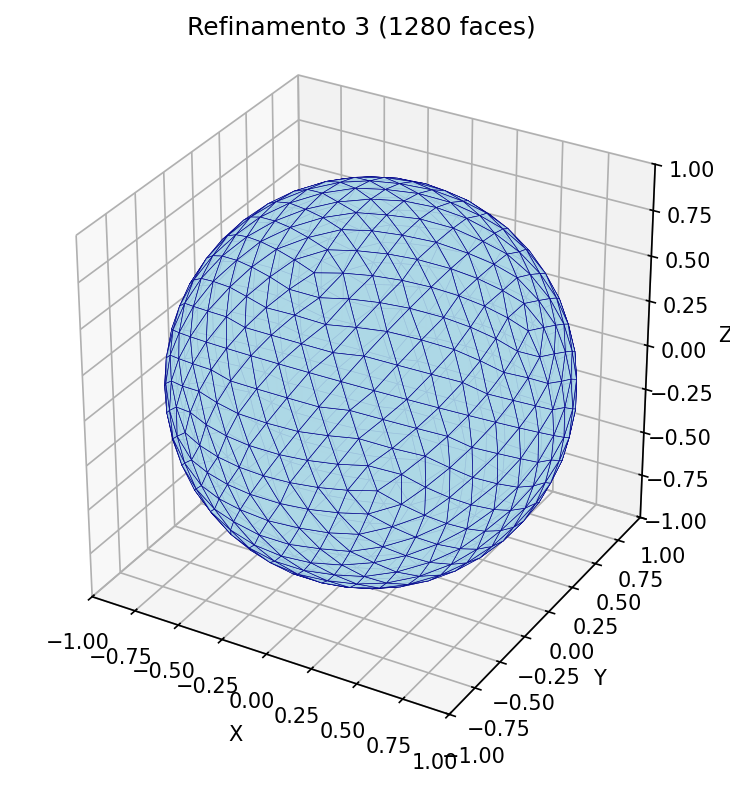
\includegraphics[width=0.48\textwidth]{../img/sphere_refine_3.png}
\end{center}
\end{column}
\end{columns}

\end{frame}

%=============================================================================
% SLIDE 3: Resultados e Conclusão
%=============================================================================
\begin{frame}{Resultados: Representação Uniforme vs Adaptativa}

\begin{columns}[T]
\begin{column}{0.48\textwidth}
\textbf{Uniforme (PyTorch + vmap):}
\begin{center}
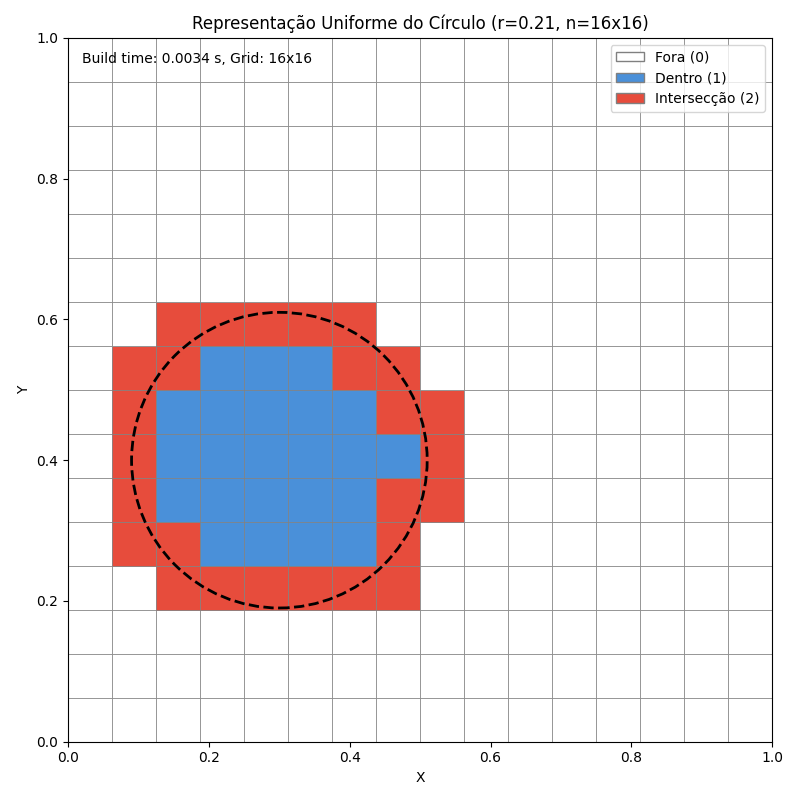
\includegraphics[width=0.48\textwidth]{../img/uniform_circle_0_grid_16.png}
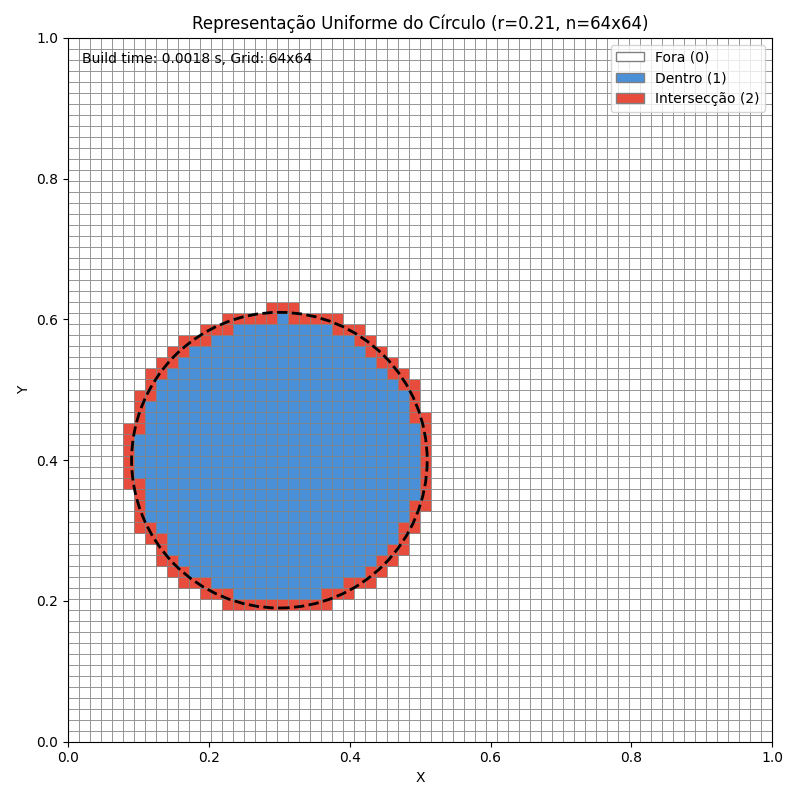
\includegraphics[width=0.48\textwidth]{../img/uniform_circle_0_grid_64.png}

\footnotesize Grade $16 \times 16$ (esq.) e $64 \times 64$ (dir.)
\end{center}
\end{column}

\begin{column}{0.48\textwidth}
\textbf{Adaptativa (Quadtree):}
\begin{center}
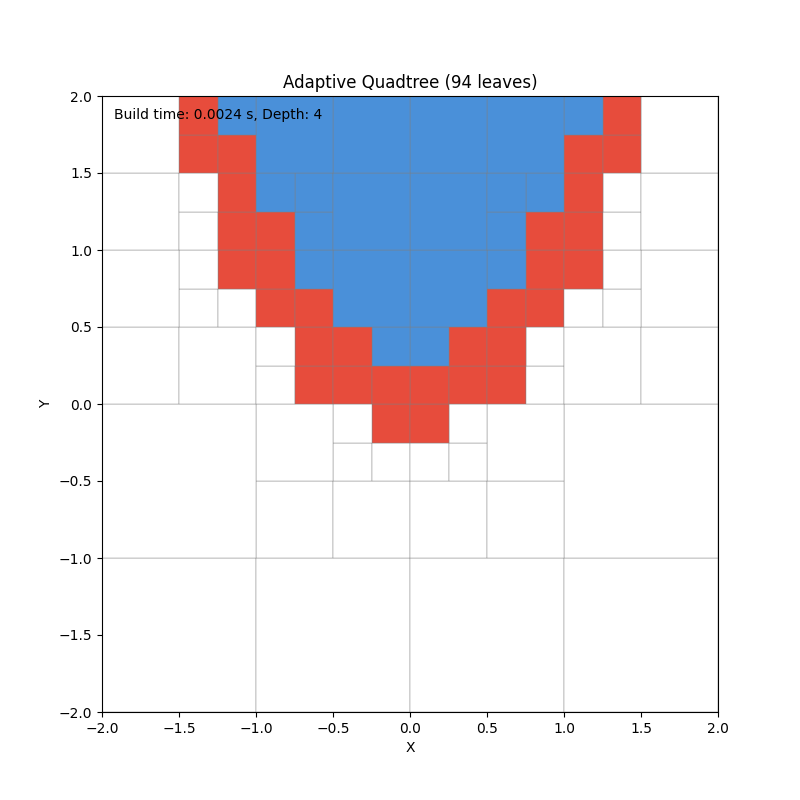
\includegraphics[width=0.48\textwidth]{../img/quadtree_parabola_0_depth_4.png}
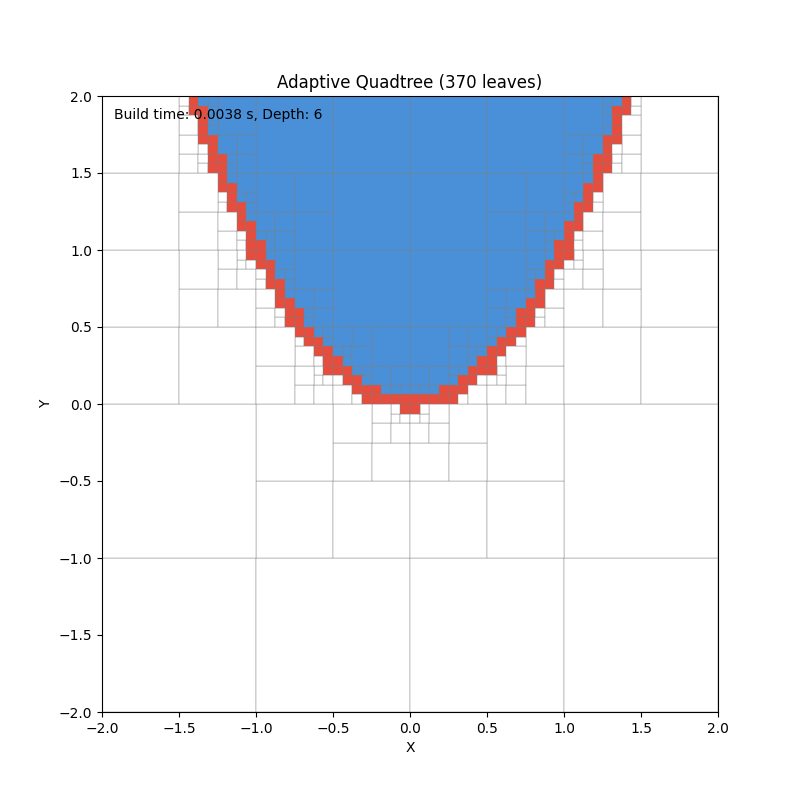
\includegraphics[width=0.48\textwidth]{../img/quadtree_parabola_0_depth_6.png}

\footnotesize Parábola: profundidade 4 (esq.) e 6 (dir.)
\end{center}
\end{column}
\end{columns}

\vspace{0.3cm}

\begin{block}{Comparação}
\textbf{Uniforme:} Todas as células do mesmo tamanho, vetorizável em GPU. \quad
\textbf{Adaptativa:} Mais eficiente em memória, foco na fronteira.
\end{block}

\end{frame}

%=============================================================================
% SLIDE 4: Conclusão
%=============================================================================
\begin{frame}{Conclusão}

\begin{columns}[T]
\begin{column}{0.55\textwidth}

\textbf{O que foi implementado:}
\begin{itemize}
    \item Representação uniforme com PyTorch/vmap (GPU)
    \item Quadtree adaptativa com animações GIF
    \item Esfera geodésica por refinamento de icosaedro
    \item Exportação para formato OBJ
\end{itemize}

\vspace{0.3cm}

\textbf{Dificuldades:}
\begin{enumerate}
    \item Adaptar para \texttt{vmap} (sem \texttt{.item()})
    \item Unificação de vértices duplicados (hash)
    \item Classificação de células para parábolas
\end{enumerate}

\end{column}

\begin{column}{0.42\textwidth}

\textbf{Arquivos Gerados:}
\begin{itemize}
    \item 72+ imagens PNG
    \item Animações GIF do processo
    \item \texttt{refined\_sphere.obj}
\end{itemize}

\vspace{0.3cm}

\textbf{Formas Testadas:}
\begin{itemize}
    \item Disco: $(0.3, 0.4)$, $r=0.21$
    \item Parábola: $y \geq x^2 + c$
    \item Icosaedro $\to$ Esfera
\end{itemize}

\end{column}
\end{columns}

\end{frame}

\end{document}
